% Created 2014-12-31 Wed 10:32
\documentclass[11pt]{article}
\usepackage[utf8]{inputenc}
\usepackage[T1]{fontenc}
\usepackage{fixltx2e}
\usepackage{graphicx}
\usepackage{longtable}
\usepackage{float}
\usepackage{wrapfig}
\usepackage{rotating}
\usepackage[normalem]{ulem}
\usepackage{amsmath}
\usepackage{textcomp}
\usepackage{marvosym}
\usepackage{wasysym}
\usepackage{amssymb}
\usepackage{hyperref}
\tolerance=1000
\date{\today}
\title{Bare Metal Provisioning with Oracle Enteprise Manager}
\hypersetup{
  pdfkeywords={},
  pdfsubject={},
  pdfcreator={Emacs 24.4.1 (Org mode 8.2.10)}}
\begin{document}

\maketitle
\tableofcontents

\section{Overview}
\label{sec-1}
\section{Conventions used in this document}
\label{sec-2}
Text to be typed in is shown in this face: \texttt{type me in}

GUI menu options will be shown connected by arrows, thus: Top -> Child1 -> Child2 -> Leaf.


\section{Current Environment}
\label{sec-3}
\section{Setup}
\label{sec-4}
The following steps need to be taken once, to allow the browser to access the Oracle Enterprise Manager (OEM) GUI, and to prepare the OEM environment for Bare Metal Provisioning (BMP).

Accessing OEM is through the OEM URL: \texttt{https://HOST:17802/em} where \texttt{HOST} is the (resolvable) hostname or ip address of the host machine. (It is assumed that the local firewall permits port 17802 to be accessed).
\subsection{Browser Certificates}
\label{sec-4-1}
Connect to the OEM URL. Your browser will likely show a security exception (the image below is shown using Firefox 31.2.0):
\begin{figure}[htb]
\centering
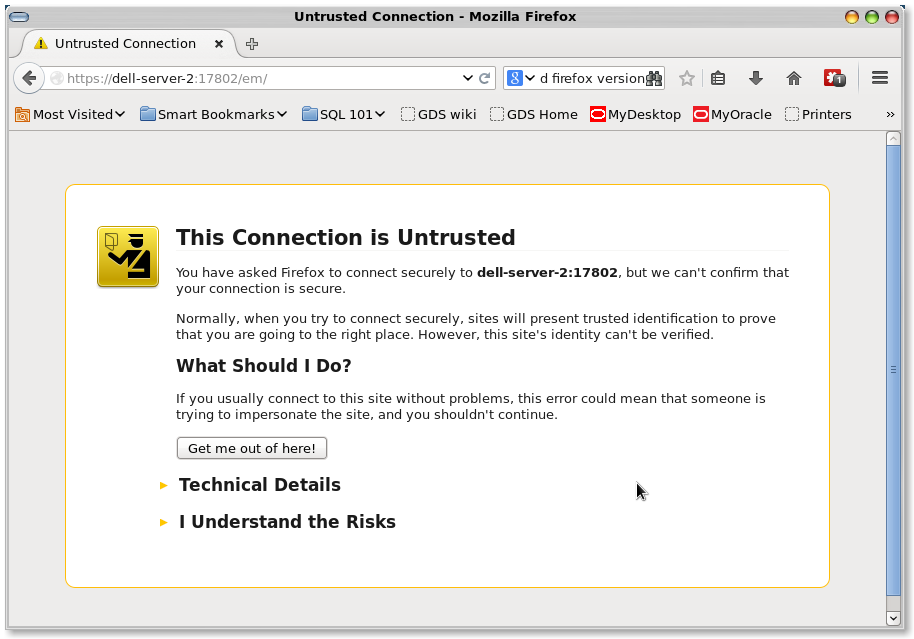
\includegraphics[width=.9\linewidth]{images/Browser_Certificate_1.png}
\caption{Initial Untrusted Certificate Screen}
\end{figure}
\clearpage
Click on the lower yellow triangle to expose the 'Add Exception\ldots{}' button:
\begin{figure}[htb]
\centering
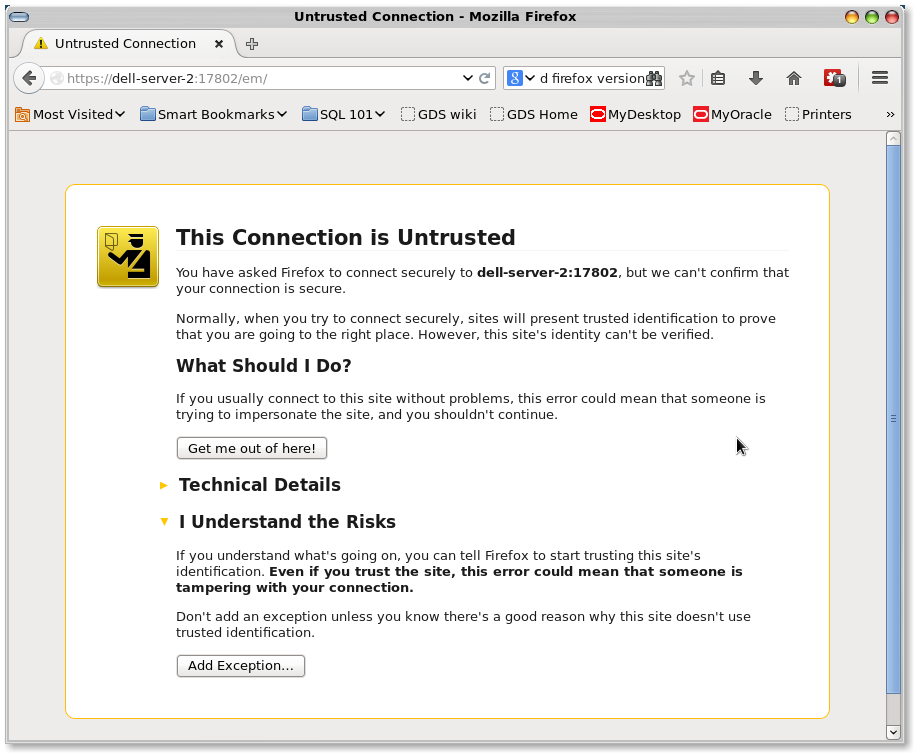
\includegraphics[width=.9\linewidth]{images/Browser_Certificate_2.png}
\caption{Untrusted Connection showing 'Add Exception\ldots{}' Button}
\end{figure}
\clearpage
Add the exception by clicking the 'Add Exception\ldots{}' button:
\begin{figure}[htb]
\centering
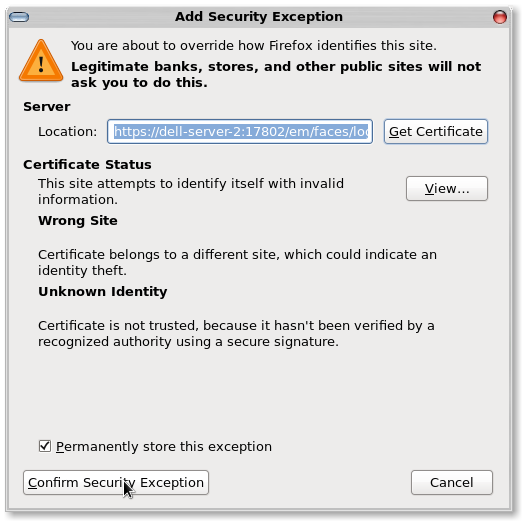
\includegraphics[width=.9\linewidth]{images/Browser_Certificate_3.png}
\caption{Add Security Exception}
\end{figure}
\clearpage
And then clicking the 'Confirm Security Exception' button. This will then take you to the OEM login window:
\begin{figure}[htb]
\centering
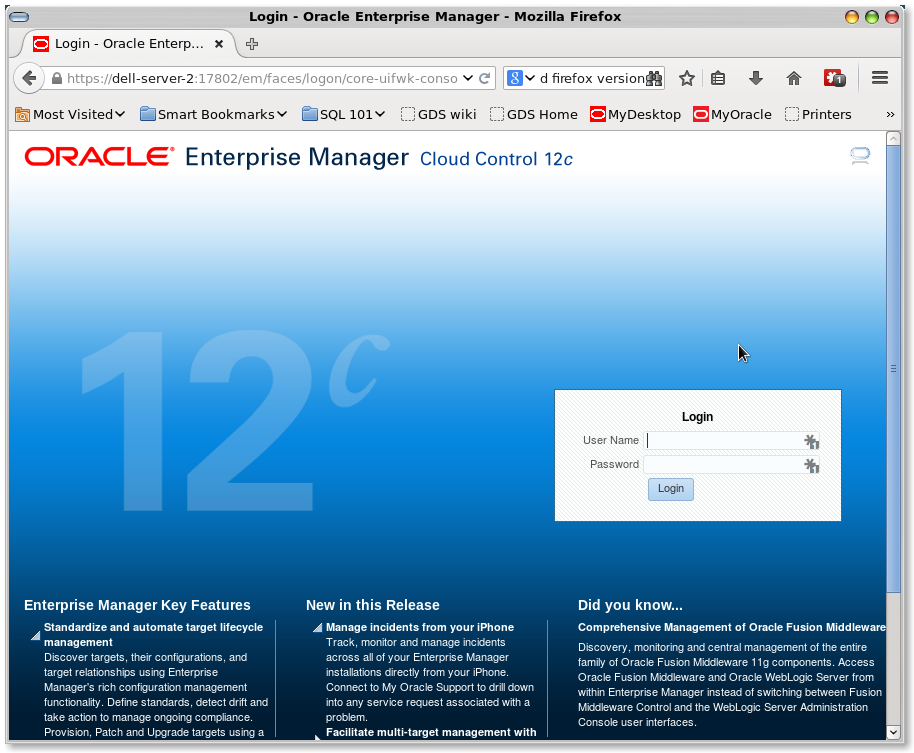
\includegraphics[width=.9\linewidth]{images/Screenshot-Login-OracleEnterpriseManager-MozillaFirefox.png}
\caption{OEM Login}
\end{figure}
\clearpage
\subsection{Oracle Enterprise Manager GUI setup}
\label{sec-4-2}
Login to OEM by accessing the OEM URL and using the name/password pair of 'sysman/Welcome1'. This will show you an 'Accessibility Preferences' page (this is \textbf{not} actually the page you'll first see! However the initial page is very similar, so hopefully this image is sufficient!):
\begin{figure}[htb]
\centering
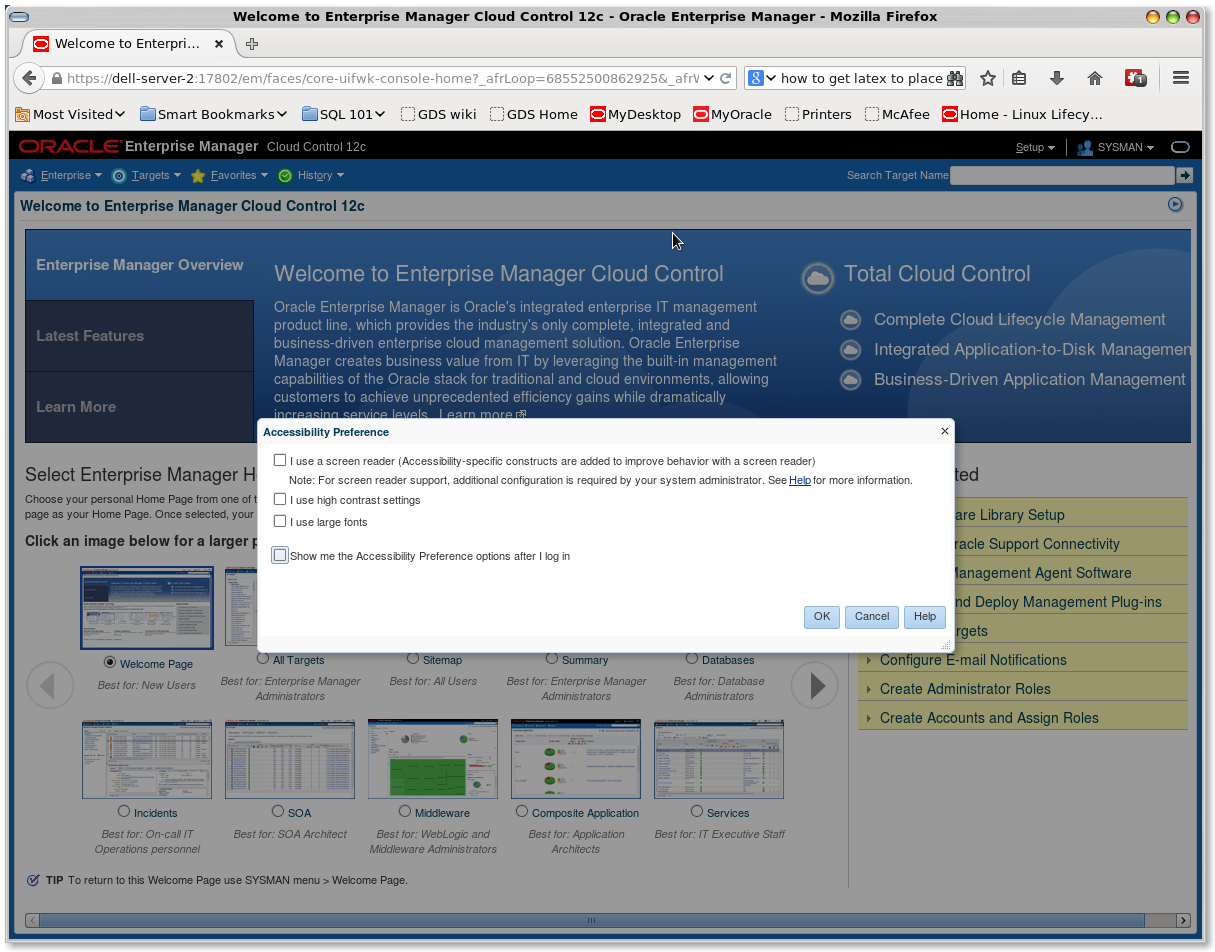
\includegraphics[width=.9\linewidth]{images/Accessibility_Preference.png}
\caption{Accessibility Preferences}
\end{figure}
\clearpage
Select the preferences for you (if any), and then OK. Your preferences are now set up and you will be taken to the 'OEM Welcome' Screen:
\begin{figure}[htb]
\centering
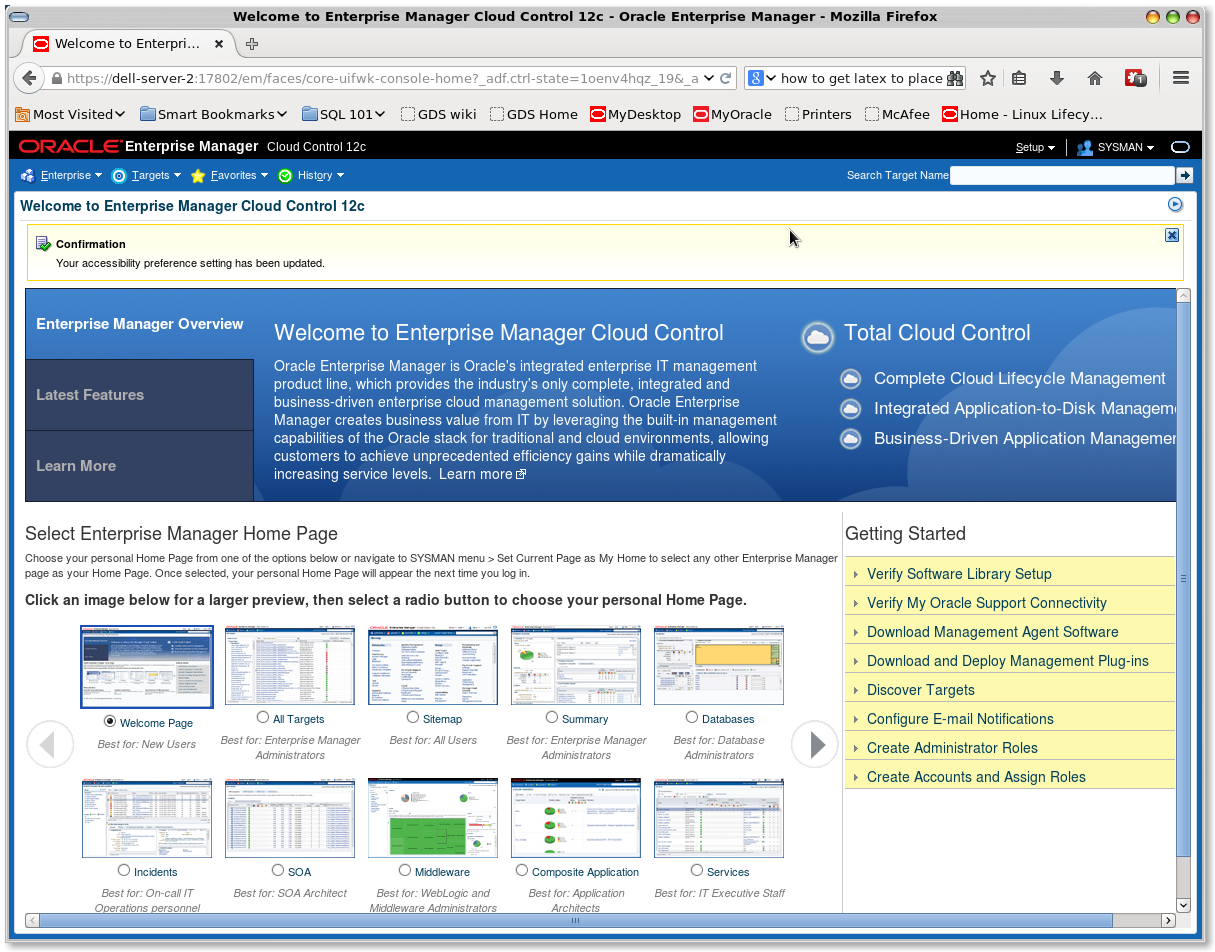
\includegraphics[width=.9\linewidth]{images/OEM_Welcome_Screen.png}
\caption{OEM Welcome Screen}
\end{figure}
\clearpage
(If you need to change these preferences you can do so using the menu Sysman -> Accessibility option)
\begin{figure}[htb]
\centering
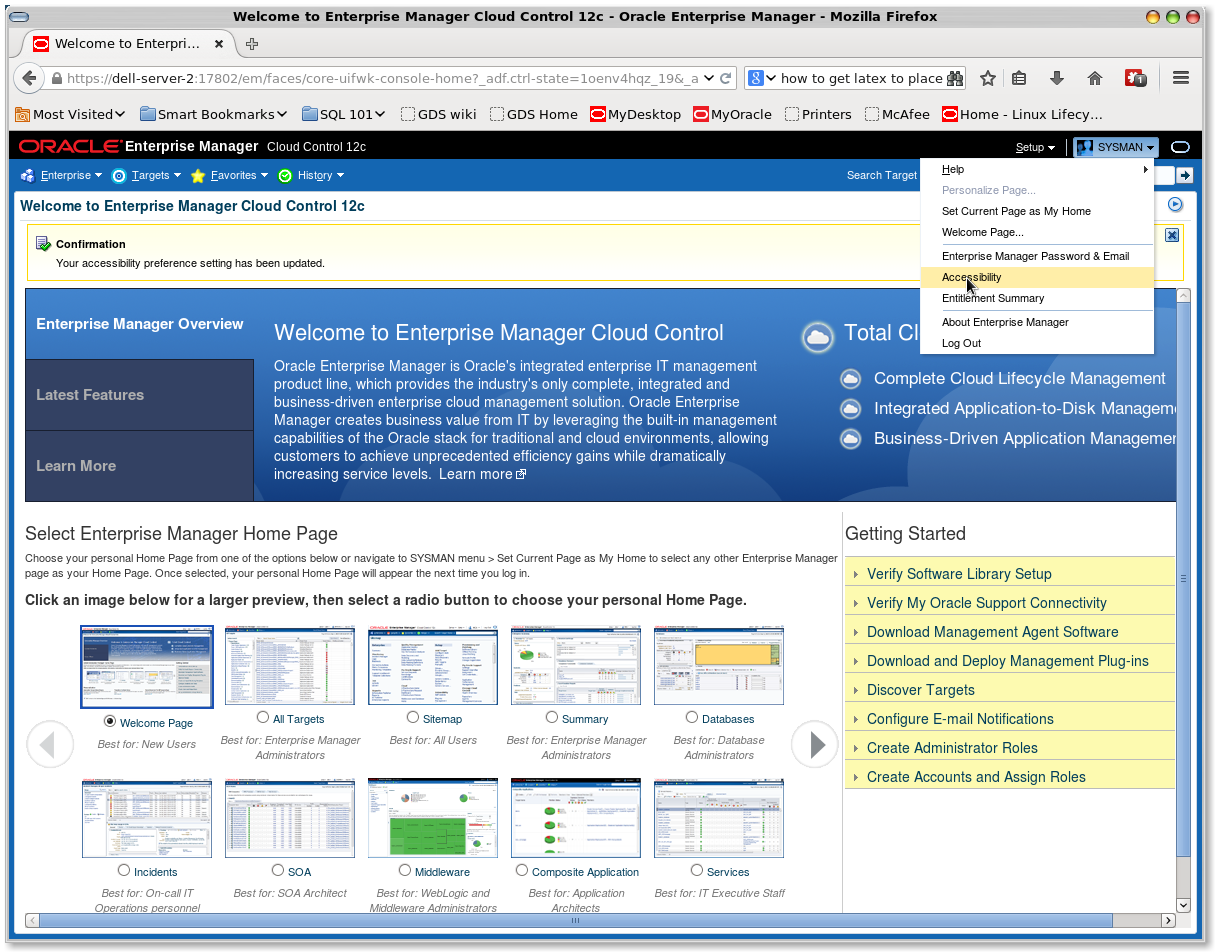
\includegraphics[width=.9\linewidth]{images/OEM_Change_Accessibility.png}
\caption{OEM Change Accessibility Menu}
\end{figure}
\clearpage
\subsection{Software Library}
\label{sec-4-3}
Bare Metal Provisioning, when run using the GUI (it can be run using the command line too), requires that at least two components be setup in the Software Library. These two components are an Operating System Component, and a Disk Component. These components will be referenced later during specific executions of BMP.
\subsubsection{Operating System Component}
\label{sec-4-3-1}
Use menu option Enterprise -> Provisioning and Patching -> Software Library to access the Software library:
\begin{figure}[htb]
\centering
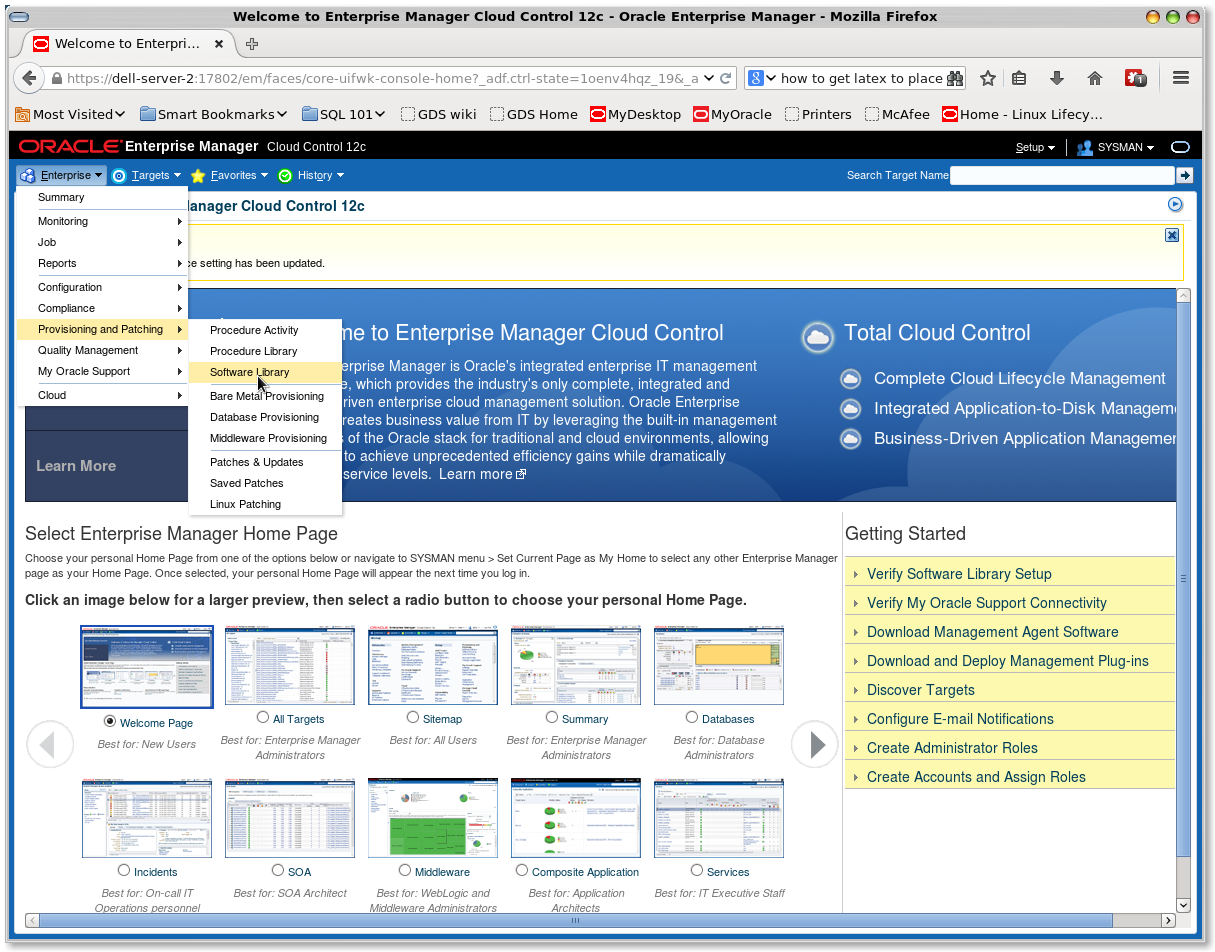
\includegraphics[width=.9\linewidth]{images/OEM_Software_Library_Access.png}
\caption{OEM Software Library Access}
\end{figure}

This will take you to the Software Library
\begin{figure}[htb]
\centering
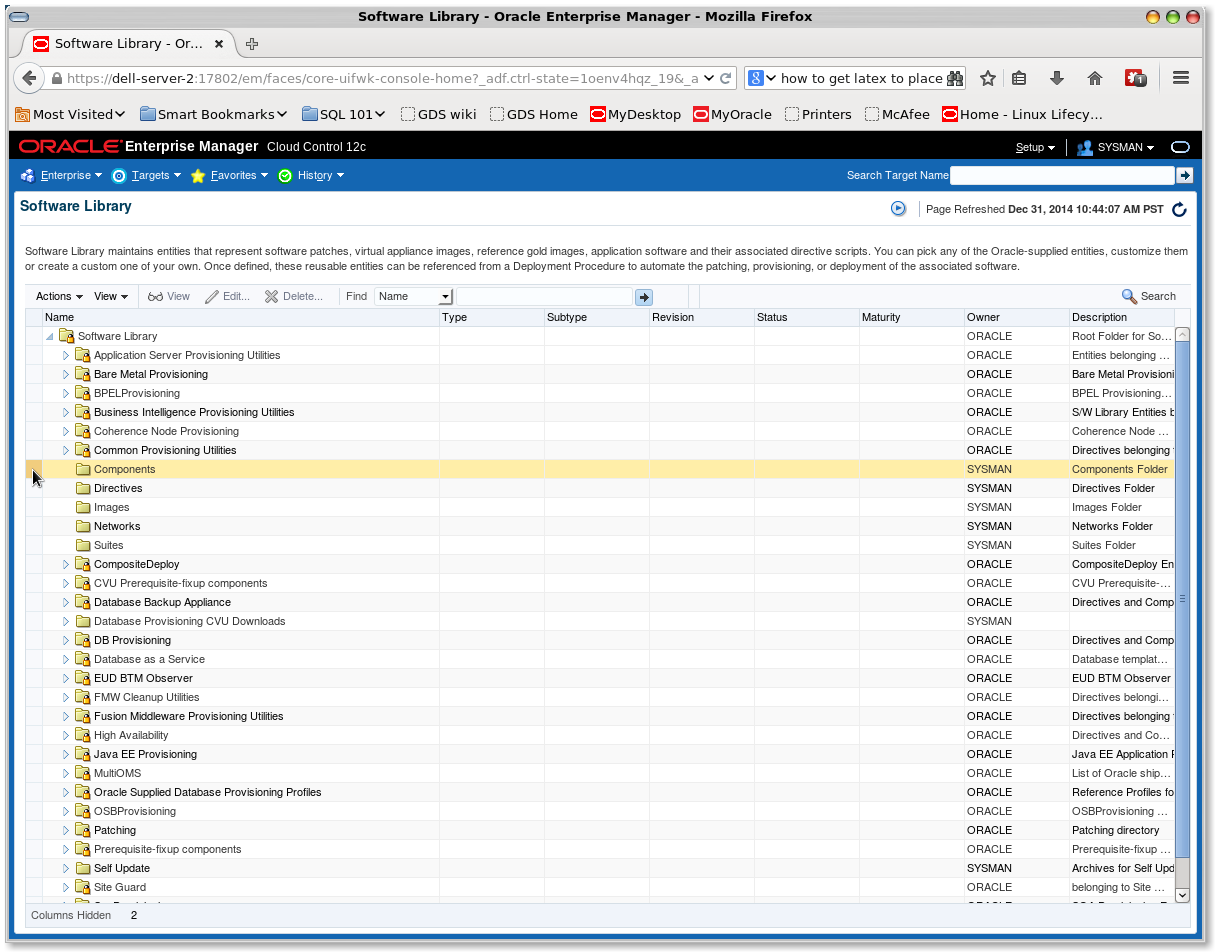
\includegraphics[width=.9\linewidth]{./images/Software_Library_1.png}
\caption{OEM Software Library}
\end{figure}
\clearpage
\subsubsection{Disk Component}
\label{sec-4-3-2}
\subsection{Bare Metal Provisioning Infrastructure}
\label{sec-4-4}
\subsection{Snapshot}
\label{sec-4-5}
\section{Demo Operation}
\label{sec-5}
% Emacs 24.4.1 (Org mode 8.2.10)
\end{document}
